\subsection{Control problem}

The full system can be seen as shown in figure \ref{fig:controlsch}.
The problem to control this system resides in finding a good motor actuation in order to stay the more close to the equilibrium as possible.
This means that the line crossing the center of gravity of the system and the wheels axis should be perpendicular to ground.

There are different posibilities to control this system.
The chosen implementation uses as error signal the aceleration in the x axis of the accelerometer, knowing that its value should be close to 0.

\begin{figure}[H]
\centering
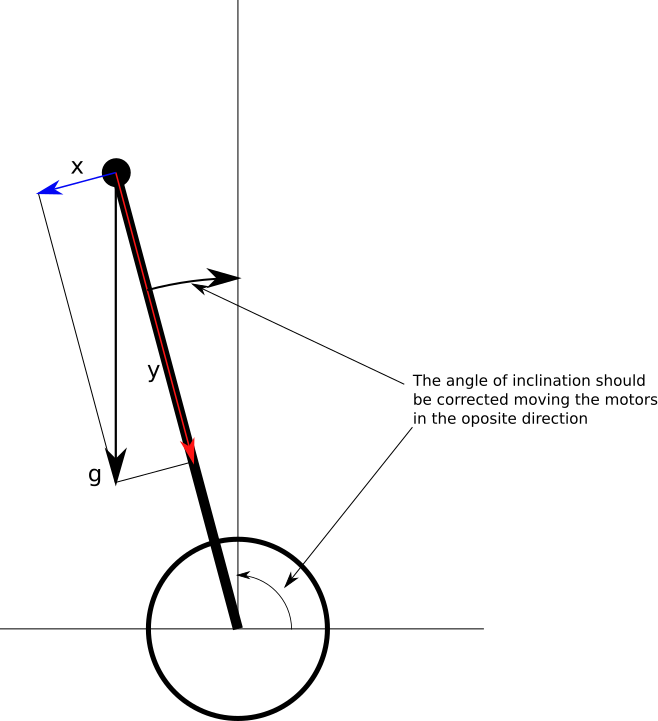
\includegraphics[width = 0.5 \textwidth]{images/segway_scheme}
\caption{Schematic of physical system.}{ The values x and y are the readings on the accelerometer for the x and y axes. As it is seen, this values are function of the angle of inclination of the segway.}
\label{fig:controlsch}
\end{figure}

In this case, it is difficult to estimate the gravity center of the robot and then a optimal PID model, but it is possible to obtain an aceptable control by tuning manually the PID.

